\section{Specifica della componente Model} {
\begin{sloppypar} {
La componente Model gestisce tutte le informazioni permanenti dell'applicazione, questa si suddivide in due categorie Client\g~ (vedi \ref{model.client}) e Server\g~ (vedi \ref{model.server}).\\

\subsection{Client}{
\label{model.client}
La sotto-componente Client\g~ si occupa della gestione dei cookie\g~ di sessione, ovvero della loro creazione, del loro recupero e della loro distruzione.
\`E formata dalle classi:
\begin{itemize}
	\item[] \texttt{mytalk.client.model.localDataUser.ManageCookies} (sez. \ref{par:CManageCookies})
	\item[] \texttt{mytalk.client.administrator.localDataUser.ManageCookies} (sez. \ref{par:AManageCookies})
\end{itemize}
		\begin{figure}[h!tbp]
		\centering
		\label{fig:modelClient}
		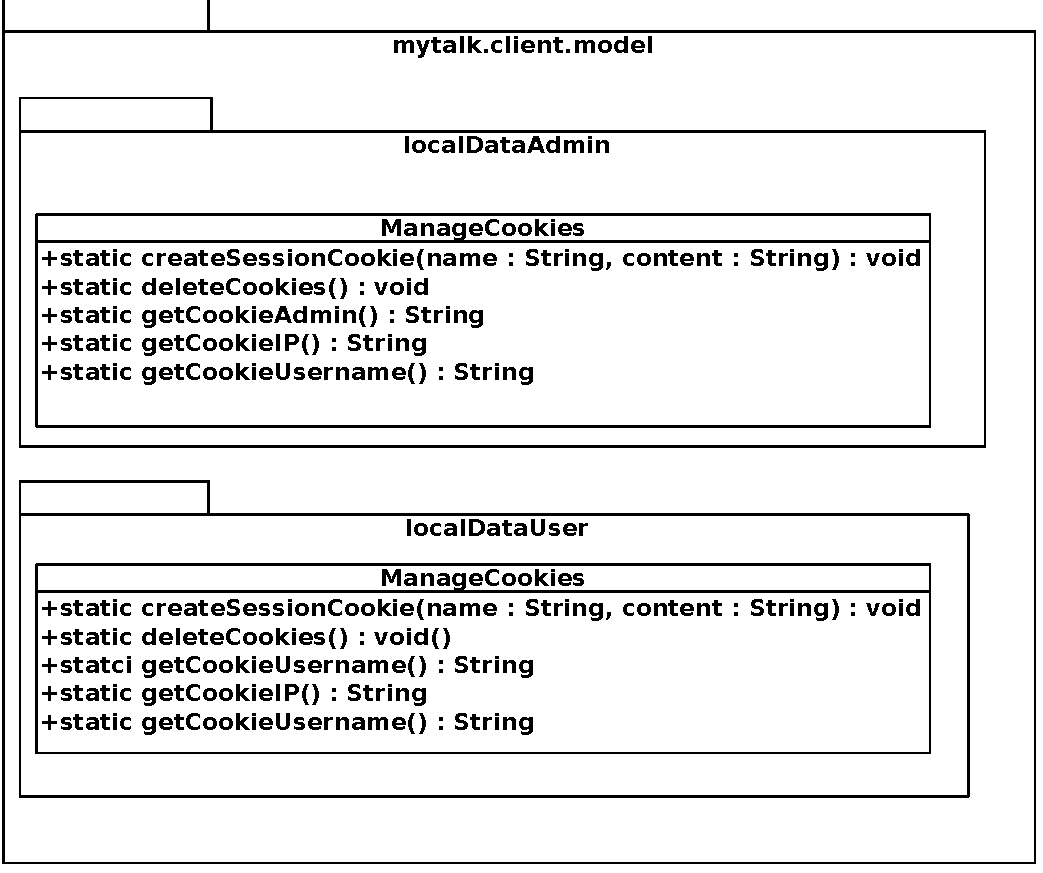
\includegraphics[scale=0.85]{\docsImg classi/modelClient.pdf}
		\caption{Diagramma delle classi del package \nolinkurl{mytalk.client.model}; dettaglio delle classi \nolinkurl{localDataAdmin.ManageCookies} e \nolinkurl{localDataUser.ManageCookies}.}	
	\end{figure}

	\subsubsection{Package mytalk.client.model.localDataUser}{
		\paragraph{ManageCookies}\label{par:CManageCookies}{
				\begin{itemize}
					\item[] \textbf{Funzione:}{\\
					Classe astratta che contiene la gestione dei cookie\g.\\
					}
				
					\item[] \textbf{Relazioni con altre componenti:}{\\
					I suoi metodi vengono usati da:
					\begin{itemize}
					\item[] \path{mytalk.client.presenter.user.logicUser.LogUserLogic};
					\item[] \path{mytalk.client.presenter.user.logicUser.RegisterLogic};
					\item[] \path{mytalk.client.presenter.user.logicUser.DataUserLogic};
					\item[] \path{mytalk.client.presenter.user.logicUser.UpdateViewLogic};
					\item[] \path{mytalk.client.presenter.administrator.logicAdmin.LogAdminLogic};
					\item[] \path{mytalk.client.presenter.administrator.serverComAdmin.WebSocketAdmin};
					\item[] \path{mytalk.client.presenter.user.serverComUser.WebSocketUser}.\\
				\end{itemize}
		
					}
					
				\item[] \textbf{Attributi:}{\\
					Nessuno.\\
					}
				
				\item[] \textbf{Metodi:}{ \\
					\texttt{+ static void createSessionCookie(String name, String content);}\\
					Crea il cookie\g~ di sessione associato all'utente. Viene richiamata due volte, una per creare un cookie\g~ con lo username e una per creare un cookie\g~ con l'indirizzo IP\g~ dell'utente.\\

					\texttt{+ static String getCookieUsername();}\\
					Ritorna il nome utente associato all'utente autenticato.\\
					
					\texttt{+ static String getCookieIP();}\\
					Ritorna l'indirizzo IP dell'utente attualmente autenticato.\\

					\texttt{+ static void deleteCookies();}\\
					Azzera e successivamente rimuove all'aggiornamento della pagina tutti i cookie\g~ associati all'utente.\\
				}
			\end{itemize}
			}
		}
	
	\subsubsection{Package mytalk.client.administrator.localDataUser}{
		\paragraph{ManageCookies}\label{par:AManageCookies}{
				\begin{itemize}
					\item[] \textbf{Funzione:}{\\
						Classe astratta che contiene la gestione dei cookie\g.\\
					}
				
					\item[] \textbf{Relazioni con altre componenti:}{\\
						I suoi metodi vengono usati da:
						\begin{itemize}
							\item[] \path{mytalk.client.presenter.administrator.logicAdmin.StatisticLogic};
							\item[] \path{mytalk.client.presenter.administrator.logicAdmin.UpdateViewLogic};\\
						\end{itemize}
		
					}
					
				\item[] \textbf{Attributi:}{\\
					Nessuno.\\
					}
				
				\item[] \textbf{Metodi:}{ \\
					\texttt{+ static void createSessionCookie(String name, String content);}\\
					Crea il cookie\g~ di sessione associato all'utente. Viene richiamata due volte, una per creare un cookie\g~ con lo username e una per creare un cookie\g~ con l'indirizzo IP\g~ dell'utente.\\

					\texttt{+ static String getCookieUsername();}\\
					Ritorna il nome utente associato all'utente autenticato.\\
					
					\texttt{+ static String getCookieIP();}\\
					Ritorna l'indirizzo IP dell'utente attualmente autenticato.\\

					\texttt{+ static void deleteCookies();}\\
					Azzera e successivamente rimuove all'aggiornamento della pagina tutti i cookie\g~ associati all'utente.\\
				}
			\end{itemize}
			}
		}
      }




\subsection{Server}{\label{model.server}
La sotto-componente Server\g~ permette la gestione e la fornitura delle informazioni ricevute da/per altre componenti in una struttura DBMS\g~ ordinata.
\`E formata dalle classi:
\begin{itemize}
	\item[] \texttt{mytalk.server.model.dao.IObjectTransfer} (sez. \ref{par:IObjectTransfer})
	\item[] \texttt{mytalk.server.model.dao.IDataAccessObject} (sez. \ref{par:IDataAccessObject})
	\item[] \texttt{mytalk.server.model.dao.ObjectTransfer} (sez. \ref{par:ObjectTransfer})
	\item[] \texttt{mytalk.server.model.dao.DataAccessObject} (sez. \ref{par:DataAccessObject})
	\item[] \texttt{mytalk.server.model.dao.DataAccessObject.User} (sez. \ref{par:DataAccessObjectUser})
	\item[] \texttt{mytalk.server.model.dao.DataAccessObject.Comm} (sez. \ref{par:DataAccessObjectComm})
	\item[] \texttt{mytalk.server.model.dao.DataAccessObject.DBDataAccess} (sez. \ref{par:DataAccessObjectDBDataAccess})
\end{itemize}


\subsubsection{Package mytalk.server.model.dao}{

	\begin{figure}[h!tbp]
		\centering
		\label{fig:figModelServer}
		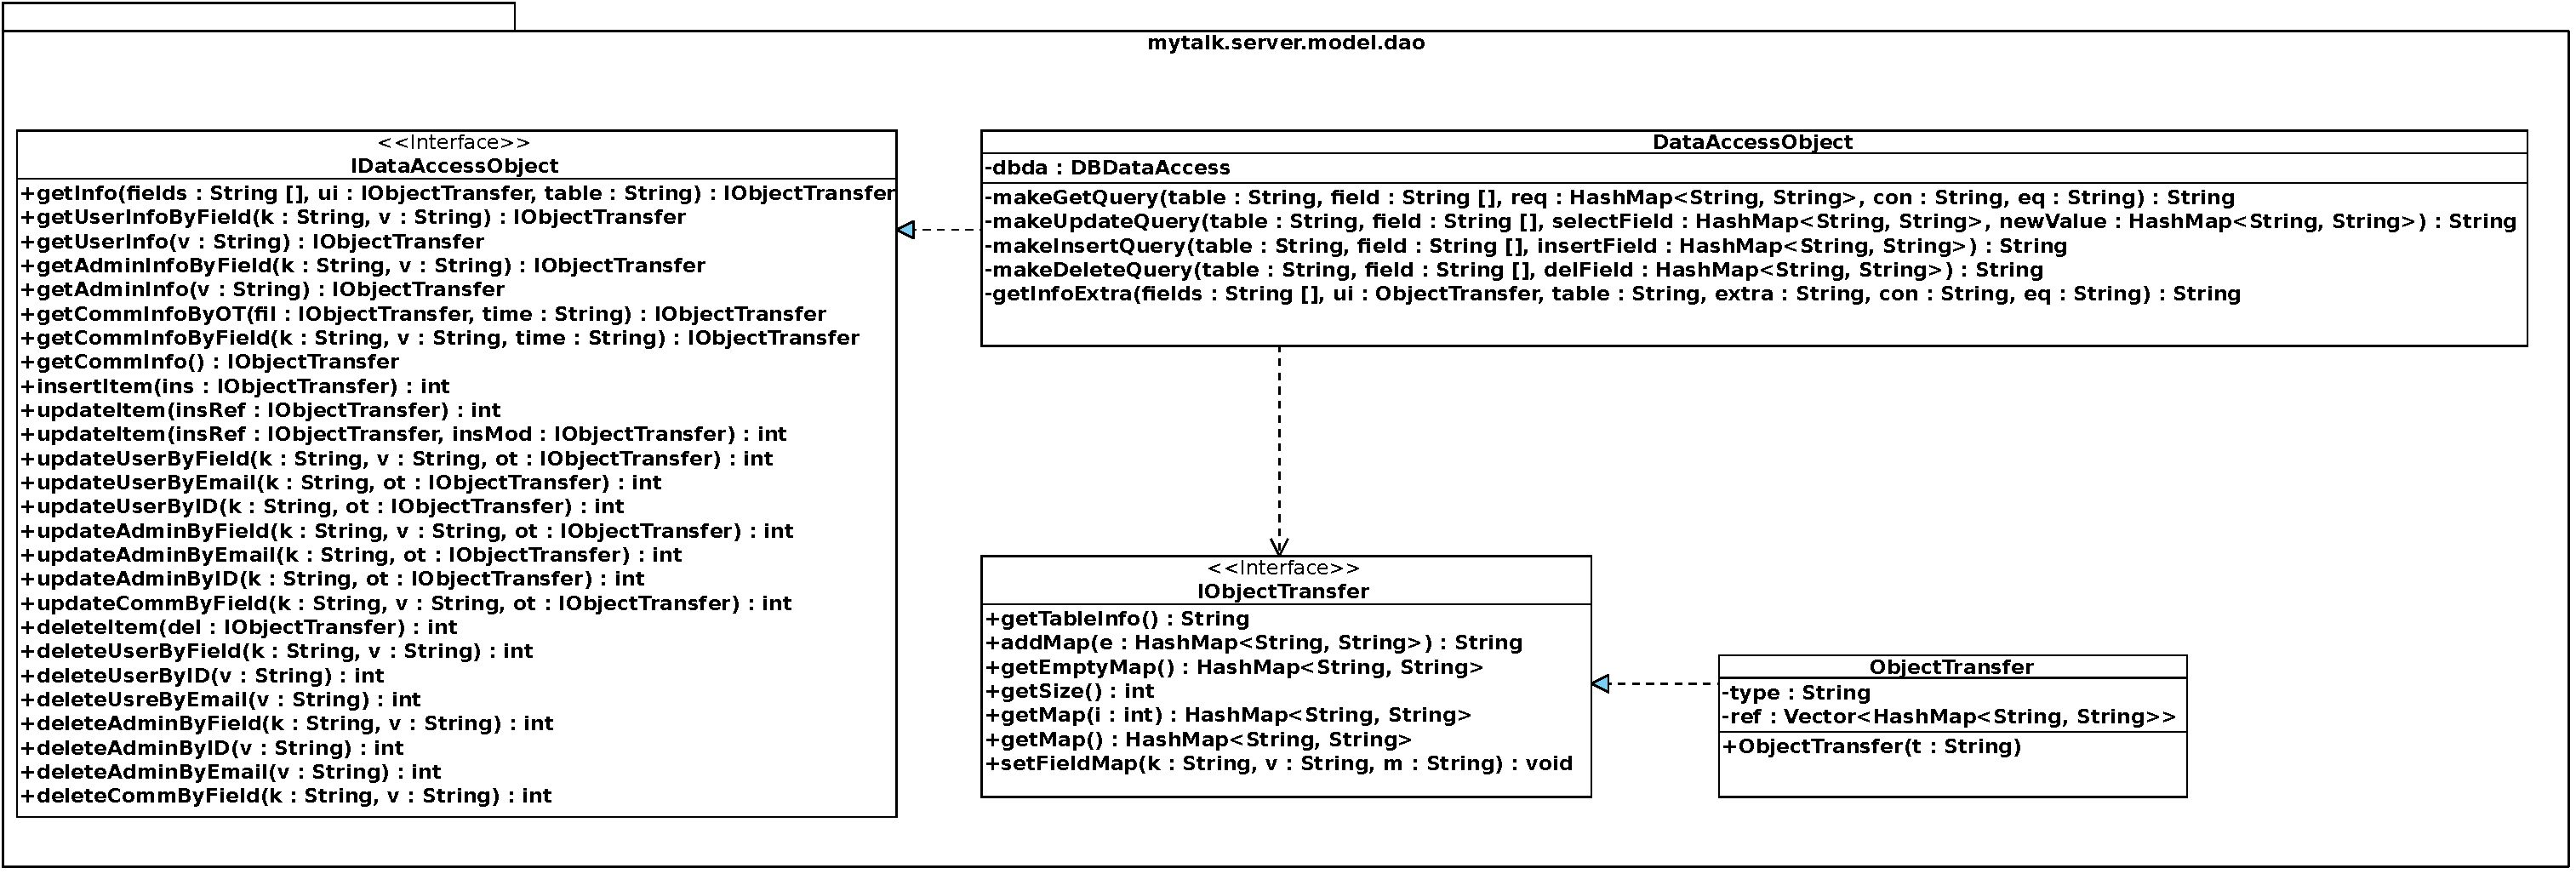
\includegraphics[scale=0.45, angle=90]{\docsImg classi/modelServer.pdf}
		\caption{Diagramma delle classi del package \nolinkurl{mytalk.server.model.dao}; dettaglio delle classi \nolinkurl{IDataAccessObject}, \nolinkurl{IObjectTransfert}, \nolinkurl{DataAccessObject} e \nolinkurl{ObjectTransfert}}	
	\end{figure}	
		
		\paragraph{IObjectTransfer}\label{par:IObjectTransfer}{
			\begin{itemize}

				\item[] \textbf{Funzione:}{\\
				Fornisce una struttura dati univoca per la gestione dei valori ricavati e da inserire nel DBMS\g.\\
				}
			
				\item[] \textbf{Relazioni con altre componenti:}{\\
				L’interfaccia è implementata da:
				\begin{itemize}
				 	\item[]	\path{mytalk.server.model.dao.ObjectTransfer}.
				\end{itemize} 		
				L’interfaccia è utilizzata da:
				\begin{itemize}
					\item[]	\path{mytalk.server.model.dao.DataAccessObject};
					\item[]	\path{mytalk.server.presenter.XMLField};
					\item[]	\path{mytalk.server.presenter.user.logicUser.ManageWSU};
					\item[]	\path{mytalk.server.presenter.admin.logicAdmin.ManageWSA}.\\
				\end{itemize}
				}
			
				\item[] \textbf{Metodi:}{ \\
				\texttt{+ String getTableInfo();}\\
				Restituisce una stringa che specifica il tipo di dati che l'oggetto contiene.\\
				
				\texttt{+ void addMap(HashMap<String, String> e);} \\ 
				Aggiunge all'oggetto una nuova mappa Hash con informazioni specifiche.\\ 
				
				\texttt{+ HashMap<String, String> getEmptyMap();} \\
				Restituisce una mappa Hash vuota dello stesso tipo dell'oggetto d'invocazione.\\ 
				
				\texttt{+ int getSize();} \\
				Restituisce il numero di mappe Hash contenute nell'oggetto.\\ 
				
				\texttt{+ HashMap<String, String> getMap(int i);} \\
				Restituisce il riferimento all' i-esima mappa Hash contenuta nell'oggetto.\\
	
				\texttt{+ HashMap<String, String> getMap();} \\
				Restituisce il riferimento alla prima mappa Hash contenuta nell'oggetto.\\
				
				\texttt{+ void setFieldMap(String k, String v, int m);} \\
				Modifica un particolare valore della m-esima mappa Hash attraverso il riferimento k ed il valore associato v.\\
				}
			\end{itemize}
			}%IObjectTransfer
			
			
			\paragraph{IDataAccessObject}\label{par:IDataAccessObject}{
			\begin{itemize}

				\item[] \textbf{Funzione:}{\\
				Esegue le operazioni richieste verso il DBMS\g~ scelto ritornandone le informazioni ricavate.\\
				}
			
				\item[] \textbf{Relazioni con altre componenti:}{\\
				L’interfaccia è implementata da:
				\begin{itemize}
				 	\item[]	\path{mytalk.server.model.dao.DataAccessObject}.
				\end{itemize} 		
				L’interfaccia è utilizzata da:
				\begin{itemize}
					\item[]	\path{mytalk.server.presenter.user.logicUser.ManageWSU};
					\item[]	\path{mytalk.server.presenter.admin.logicAdmin.ManageWSA}.\\
				\end{itemize}
				}
			
				\item[] \textbf{Metodi:}{ \\
				\texttt{+ ObjectTransfer getInfo(String[] fields, ObjectTransfer ui, String table);}\\
				Restituisce le informazioni richieste mediante i vincoli indicati dai parametri d'ingresso.\\
				
				\texttt{+ ObjectTransfer getUserInfoByField(String k, String v);} \\ 
				Restituisce le informazioni richieste relative all'utente mediante un unico vincolo relazionale chiave – valore.\\ 
				
				\texttt{+ ObjectTransfer getUserInfo(String v);} \\
				Restituisce le informazioni richieste relative all'utente mediante specifica del valore e-mail.\\ 
				
				\texttt{+ ObjectTransfer getAdminInfoByField(String k, String v);} \\
				Restituisce le informazioni richieste relative all'amministratore mediante un unico vincolo relazionale chiave – valore.\\ 
				
				\texttt{+ ObjectTransfer getAdminInfo(String v);} \\
				Restituisce le informazioni richieste relative all'amministratore mediante specifica del valore e-mail.\\
	
				\texttt{+ ObjectTransfer getCommInfoByOT(ObjectTransfer fil, String time);} \\
				Restituisce le informazioni relative alle comunicazioni filtrate dalle informazioni passate ed il tempo di interesse.\\
				
				\texttt{+ ObjectTransfer getCommInfoByField(String k, String v);} \\
				Restituisce le informazioni relative alle comunicazioni mediante un unico vincolo relazionale chiave – valore.\\
				
				\texttt{+ ObjectTransfer getCommInfo();} \\
				Restituisce le informazioni relative a tutte le comunicazioni presenti nel DBMS\g.\\

				\texttt{+ int insertItem(ObjectTransfer ins);} \\
				Inserisce nel DBMS\g~ le informazioni presenti nell'oggetto passato.\\
				
				\texttt{+ int updateItem(ObjectTransfer insRef, ObjectTransfer insMod);} \\
				Modifica le informazioni contenute nell'oggetto riferito da parametro \texttt{insRef} presenti nel DBMS\g~ aggiornandole con quelle indicate dal parametro \texttt{insMod}.\\
				
				\texttt{+ int updateUserByField(String k, String v, ObjectTransfer ot);} \\
				Modifica le informazioni dell'utente presenti nel DBMS\g, riferite dalla coppia chiave – valore passata in ingresso, aggiornandole con quelle indicate dal parametro \texttt{ot}.\\
				
				\texttt{+ int updateUserByEmail(String k, ObjectTransfer ot);} \\
				Modifica le informazioni dell'utente presenti nel DBMS\g~, riferite dal valore e-mail dato in ingresso, aggiornandole con quelle indicate dal parametro \texttt{ot}.\\
				
				\texttt{+ int updateUserByID(String k, ObjectTransfer ot);} \\
				Modifica le informazioni dell'utente presenti nel DBMS\g~, riferite dal valore ID dell'utente dato in ingresso, aggiornandole con quelle indicate dal parametro \texttt{ot}.\\
				
				\texttt{+ int updateAdminByField(String k, String v, ObjectTransfer ot);} \\
				Modifica le informazioni dell'amministratore presenti nel DBMS\g, riferite dalla coppia chiave – valore passata in ingresso, aggiornandole con quelle indicate dal parametro \texttt{ot}.\\
				
				\texttt{+ int updateAdminByEmail(String k, ObjectTransfer ot);} \\
				Modifica le informazioni dell'amministratore presenti nel DBMS\g, riferite dal valore e-mail dato in ingresso, aggiornandole con quelle indicate dal parametro \texttt{ot}.\\
				
				\texttt{+ int updateAdminByID(String k, ObjectTransfer ot);} \\
				Modifica le informazioni dell'amministratore presenti nel DBMS\g, riferite dal valore ID dell'utente dato in ingresso, aggiornandole con quelle indicate dal parametro \texttt{ot}.\\
				
				\texttt{+ int updateCommByField(String k, String v, ObjectTransfer ot);} \\
				Modifica le informazioni della comunicazione presenti nel DBMS\g, riferite dalla coppia chiave – valore passata in ingresso, aggiornandole con quelle indicate dal parametro \texttt{ot}.\\
				
				\texttt{+ int deleteItem(ObjectTransfer del);} \\
				Elimina dal DBMS\g~ le informazioni riferite dal riferimento passato.\\
				
				\texttt{+ int deleteUserByField(String k, String v);} \\
				Elimina dal DBMS\g~ le informazioni dell'utente riferite dalla coppia chiave – valore passata in ingresso.\\
				
				\texttt{+ int deleteUserByID(String v);} \\
				Elimina dal DBMS\g~ le informazioni dell'utente riferite dal valore dell'ID dato in ingresso.\\
				
				\texttt{+ int deleteUserByEmail(String v);} \\
				Elimina dal DBMS\g~ le informazioni dell'utente riferite dal valore dell'e-mail dato in ingresso.\\
				
				\texttt{+ int deleteAdminByField(String k, String v);} \\
				Elimina dal DBMS\g~ le informazioni dell'amministratore riferite dalla coppia chiave – valore passata in ingresso.\\
				
				\texttt{+ int deleteAdminByID(String v);} \\
				Elimina dal DBMS\g~ le informazioni dell'amministratore riferite dal valore dell'ID dato in ingresso.\\
				
				\texttt{+ int deleteAdminByEmail(String v);} \\
				Elimina dal DBMS\g~ le informazioni dell'amministratore riferite dal valore dell'e-mail dato in ingresso.\\
								
				\texttt{+ int deleteCommByField(String k, String v);} \\
				Elimina dal DBMS\g~ le informazioni della comunicazione riferite dalla coppia chiave – valore passata in ingresso.\\
				}
			\end{itemize}
			}%IDataAccessObject


		\paragraph{ObjectTransfer}\label{par:ObjectTransfer}{
			\begin{itemize}
			
				\item[] \textbf{Funzione:}{\\
				La classe ha la funzione di creare un riferimento univoco ai dati manipolati dal DAO.
				La sua composizione è incentrata sulla gestione di mappe Hash le quali assumono una tipologia ben  definita, a seconda dei parametri di riferimento.\\
				 }
			
			\item[] \textbf{Relazioni con altre componenti:}{\\			
				Implementa l’interfaccia: 
					\begin{itemize}
						\item[] \path{mytalk.server.model.dao.IObjectTransfer}.
					\end{itemize}
				Usa le classi:
					\begin{itemize}
				 		\item[] \path{mytalk.server.model.dao.DataAccessObject}
				 	\end{itemize}
				tramite l'interfaccia:
				 	\begin{itemize}
						\item[]\path{mytalk.server.model.dao.IDataAccessObject}.\\
					\end{itemize}
				}
				
				\item[] \textbf{Attributi:}{\\
					\texttt{- Vector<HashMap<String, String>> ref}: vettore delle mappe Hash manipolate dai metodi dell'oggetto.\\
					
					\texttt{- String type};: identifica il tipo di dati contenuti nell'oggetto.\\
				}
				
				\item[] \textbf{Metodi:}{\\
				\texttt{+ ObjectTransfer(String t);}\\
				Costruttore: inizializza l'oggetto \texttt{ObjectTransfer} del tipo specificato dalla stringa in ingresso. La tipologia resta immutabile per tutta la vita dell'oggetto.\\
				
				\texttt{+ ObjectTransfer(String t, HashMap<String, String> e);}\\
				Costruttore: inizializza l'oggetto \texttt{ObjectTransfer} del tipo specificato ed inserendo già una mappa Hash dello stesso tipo al suo interno. La tipologia resta immutabile per tutta la vita dell'oggetto.\\
				
				\texttt{+ String getTableInfo();}\\
				Restituisce una stringa che specifica il tipo di dati che l'oggetto contiene.
				Questo metodo è puramente informativo.\\
				
				\texttt{+ void addMap(HashMap<String, String> e);}\\
				Consente l'aggiunta di una nuova mappa Hash nell'oggetto a patto che essa sia dello stesso tipo dell'oggetto.\\
				
				\texttt{+ HashMap<String, String> getEmptyMap();}\\
				Consente di ottenere una mappa Hash vuota dello stesso tipo dell'oggetto \texttt{ObjectTransfer}.\\
				
				\texttt{+ int getSize();}\\
				Restituisce il numero di mappe Hash presenti nell'oggetto. Si limita a restituire il numero di elementi inseriti nel vettore che gestisce le mappe Hash.\\
				
				\texttt{+ HashMap<String, String> getMap(int i);}\\
				Restituisce la mappa Hash indicata dall'indice intero \texttt{i}. Se viene selezionato un indice negativo o maggiore del numero di mappe contenute nell'oggetto, il valore di ritorno è \texttt{null}.\\
				
				\texttt{+ HashMap<String, String> getMap();}\\
				Scorciatoia per ottenere la prima mappa Hash contenuta nell'oggetto.\\
				
				\texttt{+ void setFieldMap(String k, String v, int m);}\\
				Modifica un particolare riferimento nella mappa selezionata. L'indice \texttt{m}, che deve essere valido (\texttt{0 $\leqslant$  m \textless this.getSize() }) seleziona la mappa alla quale apportare la modifica. Il parametro \texttt{k} specifica la chiave di riferimento, mentre il parametro \texttt{v} il valore ad essa associata. Viene lasciata libertà all'utente, in quanto non viene controllato che la chiave di riferimento sia inerente al tipo della mappa Hash.\\
				}
			\end{itemize}
		}%ObjectTransfer


		\paragraph{DataAccessObject}\label{par:DataAccessObject}{
			\begin{itemize}
			
				\item[] \textbf{Funzione:}{\\
				La classe ha la funzione di interagire con il DBMS\g~ selezionato. Questa classe, inoltre raggruppa i vari riferimenti ai campi informativi, usati per gestire le informazioni ricavate dal DBMS\g, nelle due classi interne \texttt{DataAccessObject.User} e \texttt{DataAccessObject.Comm}. La gestione della connessione con il DBMS\g~ avviene mediante la classe interna \path{DataAccessObject.DBDataAccess}.
				Tutti i metodi sviluppati sono concepiti per consentire più modi per interagire con il DBMS\g~ in modo da semplificarne l'utilizzo.\\
				 }
			
			\item[] \textbf{Relazioni con altre componenti:}{\\			
				Implementa l’interfaccia: 
					\begin{itemize}
						\item[] \path{mytalk.server.model.dao.IDataAccessObject}.
					\end{itemize}
				Usa le classi:
					\begin{itemize}
				 		\item[] \path{mytalk.server.model.dao.ObjectTransfer}
				 	\end{itemize}
				e crea le classi:
					\begin{itemize}
						\item[]\path{mytalk.server.model.dao.DataAccessObject.User};
						\item[]\path{mytalk.server.model.dao.DataAccessObject.Comm};
						\item[]\path{mytalk.server.model.dao.DataAccessObject.DBDataAccess}.\\
					\end{itemize}
				}
				
				\item[] \textbf{Attributi:}{\\
					\texttt{- DBDataAccess dbda}: riferimento alla connessione al DBMS\g~ per inoltrare le query\g~ prodotte dai vari metodi.\\
				}
				
				\item[] \textbf{Metodi:}{\\
				\texttt{+ DataAccessObject();}\\
				Costruttore: crea un oggetto di tipo \texttt{DBDataAccess} per la connessione al DBMS\g.\\
				
				\texttt{- String makeGetQuery(String table, String[] field, HashMap<String, String> req, String con);}\\
				Crea e ritorna la stringa query\g~ da inoltrare al DBMS\g~ per ottenere le informazioni richieste.
				La stringa viene personalizzata dai parametri che specificano:
					\begin{itemize}
						\item[-] \texttt{table}: la tabella dove reperire le informazioni;
						\item[-] \texttt{field}: i campi informativi da reperire;
						\item[-] \texttt{req}: elenco delle coppie chiave – valore da usare come riferimento (se \texttt{null}, vengono restituite tutte le informazioni disponibili).
						\item[-] \texttt{con}: specifica il connettivo di clausola per filtrare i risultati (\texttt{AND} di default).\\
					\end{itemize}
				
				\texttt{- String makeUpdateQuery(String table, String[] field, HashMap<String, String> selectField, HashMap<String, String> newValue);}\\
				Crea e ritorna la stringa query\g~ da inoltrare al DBMS\g~ per aggiornare i valori selezionati.
				La stringa viene personalizzata dai parametri d'ingresso che specificano:
					\begin{itemize}
					\item[-] \texttt{table}: la tabella dove aggiornare le informazioni;
					\item[-] \texttt{field}: i campi informativi da aggiornare;
					\item[-] \texttt{selectField}: elenco delle coppie chiave – valore da usare come riferimento;
					\item[-] \texttt{newValue}: elenco delle coppie chiave – valore da inserire come valori da aggiornare.\\
					\end{itemize}
				
				\texttt{- String makeInsertQuery(String table, String[] field, HashMap<String, String> insertField);}\\
				Crea e ritorna la stringa query\g~ da inoltrare al DBMS\g~ per inserire le nuove informazioni inoltrate.
				La stringa viene personalizzata dai parametri d'ingresso che specificano:
					\begin{itemize}
					\item[-] \texttt{table}: la tabella dove inserire le informazioni;
					\item[-] \texttt{field}: i campi informativi da inserire;
					\item[-] \texttt{insertField}: elenco delle coppie chiave – valore da inserire come nuovi valori.\\
					\end{itemize}
				
				\texttt{- String makeDeleteQuery(String table, String[] field, HashMap<String, String> delField);}\\
				Crea e ritorna la stringa query\g~ da inoltrare al DBMS\g~ per eliminare le informazioni inoltrate.
				La stringa viene personalizzata dai parametri d'ingresso che specificano:
					\begin{itemize}
					\item[-] \texttt{table}: la tabella dove eliminare le informazioni;
					\item[-] \texttt{field}: i campi informativi da eliminare;
					\item[-] \texttt{delField}: elenco delle coppie chiave – valore da eliminare.\\
					\end{itemize}
				
				\texttt{- ObjectTransfer getInfoExtra(String[] fields, ObjectTransfer ui, String table, String extra, String con, String eq);}\\
				Restituisce, mediante oggetto \path{mytalk.server.presenter.user.logicUser.ObjectTranfer}, le informazioni richieste presenti nel DBMS\g. Il metodo estrapola i vincoli d'informazione dai parametri passati in ingresso:
				\begin{itemize}
					\item[-] \texttt{fields}: elenco chiavi per le informazioni da ricavare;
					\item[-] \texttt{ui}: valori di riferimento per filtrare le informazioni cercate;
					\item[-] \texttt{table}: tabella dove ricercare le informazioni;
					\item[-] \texttt{extra}: stringa aggiuntiva alla query\g~ che contiene parametri di filtraggio specifici;
					\item[-] \texttt{con}: stringa che specifica il connettivo di collegamento delle clausole di filtro per il parametro \texttt{WHERE} della query\g;
					\item[-] \texttt{eq}: stringa che specifica il connettivo di raffronto della clausola di filtro per il parametro \texttt{WHERE} della query\g.
				\end{itemize}
				Nel metodo viene fatta richiesta per la creazione della query\g~ d'informazione (attraverso il metodo  \texttt{makeGetQuery}) e per l'esecuzione della query\g~ (oggetto DataAccessObject.DBDataAccess).\\
				
				\texttt{+ ObjectTransfer getInfo(String[] fields, ObjectTransfer ui, String table);}\\
				Restituisce, mediante oggetto \path{mytalk.server.model.dao.ObjectTranfer}, le informazioni richieste presenti nel DBMS\g. Il metodo è un'alternativa al metodo \texttt{getInfoExtra}.\\
				
				\texttt{+ ObjectTransfer getUserInfoByField(String k, String v);}\\
				Restituisce, mediante oggetto \path{mytalk.server.model.dao.ObjectTranfer}, le informazioni richieste presenti nel DBMS\g~ relative agli utenti. Il metodo estrapola i vincoli d'informazione dai parametri passati in ingresso:
				\begin{itemize}
					\item[-] \texttt{k}: chiave di riferimento;
					\item[-] \texttt{v}: valore di riferimento per filtrare le informazioni degli utenti.
				\end{itemize}
				Questo metodo fa uso del più generico metodo \texttt{getInfo} delegandone le chiamate ai metodi interni per la query\g~ e la sua esecuzione al DBMS\g.\\
				
				\texttt{+ ObjectTransfer getUserInfo(String v);}\\
				Restituisce, mediante oggetto \texttt{mytalk.server.model.dao.ObjectTranfer}, le informazioni richieste presenti nel DBMS\g~ relative agli utenti. Il metodo estrapola i vincoli d'informazione dai parametri passati in ingresso:
				\begin{itemize}
					\item[-] \texttt{v}: valore e-mail di riferimento per selezionare l'utente.
				\end{itemize}
				Questo metodo fa uso del più generico metodo \texttt{getInfo} delegandone le chiamate ai metodi interni per la query\g~ e la sua esecuzione al DBMS\g.\\
	
				\texttt{+ ObjectTransfer getAdminInfoByField(String k, String v);}\\
				Restituisce, mediante oggetto \texttt{mytalk.server.model.dao.ObjectTranfer}, le informazioni richieste presenti nel DBMS\g~ relative agli amministratori. Il metodo estrapola i vincoli d'informazione dai parametri passati in ingresso:
				\begin{itemize}
					\item[-] \texttt{k}: chiave di riferimento;
					\item[-] \texttt{v}: valore di riferimento per filtrare le informazioni degli amministratori.
				\end{itemize}
				Questo metodo fa uso del più generico metodo getInfo delegandone le chiamate ai metodi interni per la query\g~ e la sua esecuzione al DBMS\g.\\
				
				\texttt{+ ObjectTransfer getAdminInfo(String v);}\\
				Restituisce, mediante oggetto \path{mytalk.server.model.dao.ObjectTranfer}, le informazioni richieste presenti nel DBMS\g~ relative agli amministratori. Il metodo estrapola i vincoli d'informazione dai parametri passati in ingresso:
				\begin{itemize}
					\item[-] \texttt{v}: valore e-mail di riferimento per selezionare l' amministratore.
				\end{itemize}
				Questo metodo fa uso del più generico metodo \texttt{getInfo} delegandone le chiamate ai metodi interni per la query\g~ e la sua esecuzione al DBMS\g.\\
				
				\texttt{+ ObjectTransfer getCommInfoByOT(ObjectTransfer fil, String time);}\\
				Restituisce, mediante oggetto \path{mytalk.server.model.dao.ObjectTranfer}, le informazioni richieste presenti nel DBMS\g~ relative alle statistiche di comunicazione. Il metodo estrapola i vincoli d'informazione dall'oggetto in ingresso:
				\begin{itemize}
					\item[-] \texttt{fil}: Riferimento all'oggetto \path{mytalk.server.model.dao.ObjectTranfer} contenente i parametri di filtro;
					\item[-] \texttt{time}: valore dell'arco temporale d'interessamento delle statistiche d'informazione. Se il suo valore è \texttt{null}, ritorna le informazioni disponibili seguendo i vincoli indicati.\\
				\end{itemize}
				
				\texttt{+ ObjectTransfer getCommInfoByField(String k, String v, String time);}\\
				Restituisce, mediante oggetto \path{mytalk.server.model.dao.ObjectTranfer}, le informazioni richieste presenti nel DBMS\g~ relative alle statistiche di comunicazione. Il metodo estrapola i vincoli d'informazione dai parametri passati in ingresso:
				\begin{itemize}
					\item[-] \texttt{k}: chiave di riferimento;
					\item[-] \texttt{v}: valore di riferimento per filtrare le informazioni delle comunicazioni;
					\item[-] \texttt{time}: valore dell'arco temporale d'interessamento delle statistiche d'informazione. Se il suo valore è  null, ritorna le informazioni disponibili seguendo i vincoli indicati.\\
				\end{itemize}
				
				\texttt{+ ObjectTransfer getCommInfo();}\\
				Restituisce, mediante oggetto \path{mytalk.server.model.dao.ObjectTranfer}, tutte le informazioni presenti nel DBMS\g~ relative alle statistiche di comunicazione.
				Questo metodo fa uso del più generico metodo \texttt{getCommInfoByField} delegandone le chiamate ai metodi interni per la query\g~ e la sua esecuzione al DBMS\g.\\
				
				\texttt{+ int insertItem(ObjectTransfer ins);}\\
				Inserisce nel DBMS\g~ le informazioni estrapolate dall'oggetto \path{mytalk.server.model.dao.ObjectTranfer} \texttt{ins} passato in ingresso nella tabella specificata dall'oggetto stesso.
				Il numero di ritorno si riferisce al numero di inserimenti avvenuti correttamente nel DBMS\g.
				Nel metodo viene fatta richiesta per la creazione della query\g~ di inserimento (attraverso il metodo  \texttt{makeInsertQuery}) e di eseguire la query\g~ (oggetto \texttt{DataAccessObject.DBDataAccess}).\\
				
				\texttt{+ int updateItem(ObjectTransfer insRef, ObjectTransfer insMod);}\\
				Aggiorna le informazioni selezionate presenti nel DBMS\g~ con dei nuovi valori passati.
				Il metodo estrapola i vincoli d'informazione dai parametri passati in ingresso:
				\begin{itemize}
					\item[-] \texttt{insRef}: oggetto da cui estrapolare le informazioni di vincolo per l'aggiornamento della tabella soggetta (tipologia estrapolata dall'oggetto stesso);
					\item[-] \texttt{insMod}: oggetto contenente le modifiche da apportare al DBMS\g.
				\end{itemize}
				La tipologia di tabella dove effettuare la modifica deve essere la medesima per entrambi gli oggetti.
				Il valore di ritorno si riferisce al numero di inserimenti avvenuti correttamente nel DBMS\g.
				Nel metodo viene fatta richiesta per la creazione della query\g~ di aggiornamento (attraverso il metodo  \texttt{makeUpdateQuery}) e di eseguire la query\g~ (oggetto \texttt{DataAccessObject.DBDataAccess}).\\
				
				\texttt{+ int updateUserByField(String k, String v, ObjectTransfer ot);}\\
				Aggiorna le informazioni selezionate relative agli utenti presenti nel DBMS\g~ con dei nuovi valori passati.
				Il metodo estrapola i vincoli d'informazione dai parametri passati:
				\begin{itemize}
					\item[-] \texttt{k}: chiave di riferimento;
					\item[-] \texttt{v}: valore di riferimento per filtrare le informazioni degli utenti;
					\item[-] \texttt{ot}: oggetto contenente le modifiche da apportare al DBMS\g.
				\end{itemize}
				Il valore  di ritorno si riferisce al numero di inserimenti avvenuti correttamente nel DBMS\g.
				Questo metodo fa uso del più generico metodo \texttt{updateItem} delegandone le chiamate ai metodi interni per la query\g~ e la sua esecuzione al DBMS\g.\\
				
				\texttt{+ int updateUserByEmail(String k, ObjectTransfer ot);}\\
				Aggiorna le informazioni selezionate relative agli utenti presenti nel DBMS\g~ con dei nuovi valori passati.
				Il metodo estrapola i vincoli d'informazione dai parametri passati:
				\begin{itemize}
					\item[-] \texttt{k}: valore di riferimento dell'e-mail per filtrare le informazioni degli utenti;
					\item[-] \texttt{ot}: oggetto contenente le modifiche da apportare al DBMS\g.
				\end{itemize}
				Il valore  di ritorno si riferisce al numero di inserimenti avvenuti correttamente nel DBMS\g.
				Questo metodo fa uso del più generico metodo \texttt{updateItem} delegandone le chiamate ai metodi interni per la query\g~ e la sua esecuzione al DBMS\g.\\
				
				\texttt{+ int updateUserByID(String k, ObjectTransfer ot);}\\
				Aggiorna le informazioni selezionate relative agli utenti presenti nel DBMS\g~ con dei nuovi valori passati.
				Il metodo estrapola i vincoli d'informazione dai parametri passati:
				\begin{itemize}
					\item[-] \texttt{k}: valore di riferimento dell'ID per filtrare le informazioni degli utenti;
					\item[-] \texttt{ot}: oggetto d'ingresso contenente le modifiche da apportare al DBMS\g.
				\end{itemize}
				Il valore  di ritorno si riferisce al numero di inserimenti avvenuti correttamente nel DBMS\g.
				Questo metodo fa uso del più generico metodo \texttt{updateItem} delegandone le chiamate ai metodi interni per la query\g~ e la sua esecuzione al DBMS\g.\\
				
				\texttt{+ int updateAdminByField(String k, String v, ObjectTransfer ot);}\\
				Aggiorna le informazioni selezionate relative agli amministratori presenti nel DBMS\g~ con dei nuovi valori passati.
				Il metodo estrapola i vincoli d'informazione dai parametri passati:
				\begin{itemize}
					\item[-] \texttt{k}: chiave di riferimento;
					\item[-] \texttt{v}: valore di riferimento per filtrare le informazioni degli amministratori;
					\item[-] \texttt{ot}: oggetto d'ingresso contenente le modifiche da apportare al DBMS\g.
				\end{itemize}
				Il valore  di ritorno si riferisce al numero di inserimenti avvenuti correttamente nel DBMS\g.
				Questo metodo fa uso del più generico metodo \texttt{updateItem} delegandone le chiamate ai metodi interni per la query\g~ e la sua esecuzione al DBMS\g.\\
				
				\texttt{+ int updateAdminByEmail(String k, ObjectTransfer ot);}\\
				Aggiorna le informazioni selezionate relative agli amministratori presenti nel DBMS\g~ con dei nuovi valori passati.
				Il metodo estrapola i vincoli d'informazione dai parametri passati:
				\begin{itemize}
					\item[-] \texttt{k}: valore di riferimento dell'e-mail per filtrare le informazioni degli amministratori;
					\item[-] \texttt{ot}: oggetto d'ingresso contenente le modifiche da apportare al DBMS\g.
				\end{itemize}
				Il valore  di ritorno si riferisce al numero di inserimenti avvenuti correttamente nel DBMS\g.
				Questo metodo fa uso del più generico metodo \texttt{updateItem} delegandone le chiamate ai metodi interni per la query\g~ e la sua esecuzione al DBMS\g.\\
				
				\texttt{+ int updateAdminByID(String k, ObjectTransfer ot);}\\
				Aggiorna le informazioni selezionate relative agli amministratori presenti nel DBMS\g~ con dei nuovi valori passati.
				Il metodo estrapola i vincoli d'informazione dai parametri passati:
				\begin{itemize}
					\item[-] \texttt{k}: valore di riferimento dell'ID per filtrare le informazioni degli amministratori;
					\item[-] \texttt{ot}: oggetto d'ingresso contenente le modifiche da apportare al DBMS\g.
				\end{itemize}
				Il valore  di ritorno si riferisce al numero di inserimenti avvenuti correttamente nel DBMS\g.
				Questo metodo fa uso del più generico metodo \texttt{updateItem} delegandone le chiamate ai metodi interni per la query\g~ e la sua esecuzione al DBMS\g.\\
				
				\texttt{+ int updateCommByField(String k, String v, ObjectTransfer ot);}\\
				Aggiorna le informazioni selezionate relative alle statistiche di comunicazione presenti nel DBMS\g~ con dei nuovi valori passati.
				Il metodo estrapola i vincoli d'informazione dai parametri passati:
				\begin{itemize}
					\item[-] \texttt{k}: chiave di riferimento;
					\item[-] \texttt{v}: valore di riferimento per filtrare le informazioni delle comunicazioni;
					\item[-] \texttt{ot}: oggetto d'ingresso contenente le modifiche da apportare al DBMS\g.
				\end{itemize}
				Il valore  di ritorno si riferisce al numero di inserimenti avvenuti correttamente nel DBMS\g.
				Questo metodo fa uso del più generico metodo \texttt{updateItem} delegandone le chiamate ai metodi interni per la query\g~ e la sua esecuzione al DBMS\g.\\
				
				\texttt{+ int deleteItem(ObjectTransfer del);}\\
				Elimina le informazioni selezionate presenti nel DBMS\g.
				Il metodo estrapola i vincoli di selezione dal parametro del quale ricava anche la tabella su cui eseguire l'operazione.
				Il valore  di ritorno si riferisce al numero di inserimenti avvenuti correttamente nel DBMS\g.
				Nel metodo viene fatta richiesta per la creazione della query\g~ di eliminazione (attraverso il metodo  \texttt{makeDeleteQuery}), la query\g~ viene eseguita attraverso (oggetto \texttt{DataAccessObject.DBDataAccess}).\\
				
				\texttt{+ int deleteUserByField(String k, String v);}\\
				Elimina le informazioni relative agli utenti presenti nel DBMS\g.
				Il metodo estrapola i vincoli d'informazione dai parametri passati:
				\begin{itemize}
					\item[-] \texttt{k}: chiave di riferimento;
					\item[-] \texttt{v}: valore di riferimento per filtrare le informazioni degli utenti.
				\end{itemize}
				Il valore  di ritorno si riferisce al numero di inserimenti avvenuti correttamente nel DBMS\g.
				Questo metodo fa uso del più generico metodo \texttt{deleteItem} delegandone le chiamate ai metodi interni per la query\g~ e la sua esecuzione al DBMS\g.\\
				
				\texttt{+ int deleteUserByID(String v);}\\
				Elimina le informazioni relative agli utenti presenti nel DBMS\g~ mediante parametro \texttt{v} che indica l'ID univoco.
				Il valore  di ritorno si riferisce al numero di inserimenti avvenuti correttamente nel DBMS\g.
				Questo metodo fa uso del più generico metodo \texttt{deleteItem} delegandone le chiamate ai metodi interni per la query\g~ e la sua esecuzione al DBMS\g.\\
				
				\texttt{+ int deleteUserByEmail(String v);}\\
				Elimina le informazioni relative agli utenti presenti nel DBMS\g~ mediante parametro \texttt{v} che indica l'indirizzo e-mail univoco.
				Il valore  di ritorno si riferisce al numero di inserimenti avvenuti correttamente nel DBMS\g.
				Questo metodo fa uso del più generico metodo \texttt{deleteItem} delegandone le chiamate ai metodi interni per la query\g~ e la sua esecuzione al DBMS\g.\\
				
				\texttt{+ int deleteAdminByField(String k, String v);}\\
				Elimina le informazioni relative agli amministratori presenti nel DBMS\g.
				Il metodo estrapola i vincoli d'informazione dai parametri passati:
				\begin{itemize}
					\item[-] \texttt{k}: chiave di riferimento;
					\item[-] \texttt{v}: valore di riferimento per filtrare le informazioni degli amministratori.
				\end{itemize}
				Il valore  di ritorno si riferisce al numero di inserimenti avvenuti correttamente nel DBMS\g.
				Questo metodo fa uso del più generico metodo \texttt{deleteItem} delegandone le chiamate ai metodi interni per la query\g~ e la sua esecuzione al DBMS\g.\\
				
				\texttt{+ int deleteAdminByID(String v);}\\
				Elimina le informazioni relative agli amministratori presenti nel DBMS\g~ mediante parametro \texttt{v} che indica l'ID univoco.
				Il valore  di ritorno si riferisce al numero di inserimenti avvenuti correttamente nel DBMS\g.
				Questo metodo fa uso del più generico metodo \texttt{deleteItem} delegandone le chiamate ai metodi interni per la query\g~ e la sua esecuzione al DBMS\g.\\
				
				\texttt{+ int deleteAdminByEmail(String v);}\\
				Elimina le informazioni relative agli amministratori presenti nel DBMS\g~ mediante parametro \texttt{v} che indica l'indirizzo e-mail univoco.
				Il valore  di ritorno si riferisce al numero di inserimenti avvenuti correttamente nel DBMS\g.
				Questo metodo fa uso del più generico metodo \texttt{deleteItem} delegandone le chiamate ai metodi interni per la query\g~ e la sua esecuzione al DBMS\g.\\
				
				\texttt{+ int deleteCommByField(String k, String v);}\\
				Elimina le informazioni relative alle statistiche di comunicazione presenti nel DBMS\g.
				Il metodo estrapola i vincoli d'informazione dai parametri passati:
				\begin{itemize}
					\item[-] \texttt{k}: chiave di riferimento;
					\item[-] \texttt{v}: valore di riferimento per filtrare le informazioni delle comunicazioni.
				\end{itemize}
				Il valore  di ritorno si riferisce al numero di inserimenti avvenuti correttamente nel DBMS\g.
				Questo metodo fa uso del più generico metodo \texttt{deleteItem} delegandone le chiamate ai metodi interni per la query\g~ e la sua esecuzione al DBMS\g.\\
				}
			\end{itemize}
		}%DataAccessObject


		\paragraph{DataAccessObject.User}\label{par:DataAccessObjectUser}{
			\begin{itemize}
			
				\item[] \textbf{Funzione:}{\\
				La classe ha la funzione di racchiudere tutti i valori di riferimento relativi alle informazioni degli utenti e degli amministratori gestite nel DBMS\g~ e nell'oggetto di scambio \texttt{mytalk.server.model.dao.ObjectTranfer}.\\
				 }
			
			\item[] \textbf{Relazioni con altre componenti:}{\\			
				La classe è implementata da:
					\begin{itemize}
						\item[] \path{mytalk.server.model.dao.DataAccessObject};
						\item[] \path{mytalk.server.model.dao.ObjectTransfer};
						\item[] \path{mytalk.server.presenter.XMLField};
						\item[]	\path{mytalk.server.presenter.user.logicUser.ManageWSU};
						\item[]	\path{mytalk.server.presenter.admin.logicAdmin.ManageWSA}.\\
					\end{itemize}
				}
				
				\item[] \textbf{Attributi:}{\\
					\texttt{+ static final String user}: riferimento alla tabella degli utenti del DBMS\g.\\
					
					\texttt{+ static final String admin}: riferimento alla tabella degli amministratori del DBMS\g.\\
					
					\texttt{+ static final String fieldAID}: riferimento al valore ID della tabella degli amministratori.\\
					
					\texttt{+ static final String fieldUID}: riferimento al valore ID della tabella degli utenti.\\
					
					\texttt{+ static final String fieldPsw}: riferimento al valore password nelle tabelle degli utenti ed amministratori.\\
					
					\texttt{+ static final String fieldName}: riferimento al valore nome nelle tabelle degli utenti ed amministratori.\\
					
					\texttt{+ static final String fieldSName}: riferimento al valore cognome nelle tabelle degli  utenti ed amministratori.\\
					
					\texttt{+ static final String fieldMail}: riferimento al valore dell'indirizzo e-mail nelle tabelle utenti ed amministratori.\\
					
					\texttt{+ static final String fieldDtReg}: riferimento al valore della data di registrazione nelle tabelle degli utenti ed amministratori.\\
					
					\texttt{+ static final String fieldSociety}: riferimento al valore dell'azienda nelle tabelle degli utenti ed amministratori.\\
					
					\texttt{+ static final String fieldTel}: riferimento al valore del numero telefonico nelle tabelle degli utenti ed amministratori.\\
					
					\texttt{+ static final String fieldOnline}: riferimento al valore online nelle tabelle degli utenti.\\
					
					\texttt{+ static final String fieldIP}: riferimento al valore IP nelle tabelle degli utenti.\\
					
					\texttt{+ static final String[] fieldUser}: array che raccoglie tutte le informazioni relative agli utenti presenti nel DBMS\g.\\
					
					\texttt{+ static final String[] fieldAdmin}: array che raccoglie tutte le informazioni relative agli amministratori presenti nel DBMS\g.\\
				}
			\end{itemize}
		}%DataAccessObject.User
		
		
		\paragraph{DataAccessObject.Comm}\label{par:DataAccessObjectComm}{
			\begin{itemize}
			
				\item[] \textbf{Funzione:}{\\
				La classe ha la funzione di racchiudere tutti i valori relativi alle informazioni   statistiche delle comunicazioni gestite nel DBMS\g~ e nell'oggetto di scambio \texttt{mytalk.server.model.dao.ObjectTranfer}.\\
				 }
			
			\item[] \textbf{Relazioni con altre componenti:}{\\			
				La classe è implementata da:
					\begin{itemize}
						\item[] \path{mytalk.server.model.dao.DataAccessObject};
						\item[] \path{mytalk.server.model.dao.ObjectTransfer};
						\item[] \path{mytalk.server.presenter.XMLField};
						\item[]	\path{mytalk.server.presenter.user.logicUser.ManageWSU};
						\item[]	\path{mytalk.server.presenter.admin.logicAdmin.ManageWSA}.\\
					\end{itemize}
				}
				
				\item[] \textbf{Attributi:}{\\
					\texttt{+ static final String comm}: riferimento alla tabella  delle statistiche di comunicazione nel DBMS\g.\\

					\texttt{+ static final String fieldCID}: riferimento al valore ID della tabella delle comunicazioni.\\
					
					\texttt{+ static final String fieldUSender}: riferimento all'indirizzo e-mail dell'utente mittente nelle tabelle delle comunicazioni.\\
					
					\texttt{+ static final String fieldUReceiver}: riferimento all'indirizzo e-mail dell'utente destinatario nelle tabelle delle comunicazioni.\\
					
					\texttt{+ static final String fieldByteIn}: riferimento al numero di byte trasmessi nelle tabelle delle comunicazioni.\\
					
					\texttt{+ static final String fieldPack}: riferimento al numero di pacchetti scambiati nelle tabelle delle comunicazioni.\\
					
					\texttt{+ static final String fieldPackLost}: riferimento al numero di pacchetti persi nelle tabelle delle comunicazioni.\\
					
					\texttt{+ static final String fieldStart}: riferimento alla data di inizio della chiamata nelle tabelle delle comunicazioni.\\
					
					\texttt{+ static final String fieldEnd}: riferimento alla data di termine della chiamata nelle tabelle delle comunicazioni.\\
					
					\texttt{+ static final String fieldGS}: riferimento al valore di gradimento dell'utente mittente nelle tabelle delle comunicazioni.\\
					
					\texttt{+ static final String fieldGR}: riferimento al valore di gradimento dell'utente destinatario nelle tabelle delle comunicazioni.\\
					
					\texttt{+ static final String[] fieldComm}: array che raccoglie tutti valori di riferimento per le informazioni relative alla comunicazione presenti nel DBMS\g.\\
				}
			\end{itemize}
		}%DataAccessObject.Comm
		
		
		\paragraph{DataAccessObject.DBDataAccess}\label{par:DataAccessObjectDBDataAccess}{
			\begin{itemize}
			
				\item[] \textbf{Funzione:}{\\
				La classe ha la funzione di gestire la connessione verso il DBMS\g~ con i parametri indicati nel file \path{mytalk.server.model.dao.DBAccess.xml}.\\
				 }
			
			\item[] \textbf{Relazioni con altre componenti:}{\\			
				La classe è implementata da: 
					\begin{itemize}
						\item[] \path{mytalk.server.model.dao.DataAccessObject}.\\
					\end{itemize}
				}
				
				\item[] \textbf{Attributi:}{\\
					\texttt{- String user}: riferimento al valore dell'utente abilitato alla connessione al DBMS\g.\\
					
					\texttt{- String psw}: riferimento al valore della password utente abilitato alla connessione al DBMS\g.\\
					
					\texttt{- String driver}: riferimento del driver usato dal programma per la connessione al DBMS\g.\\
					
					\texttt{- String url}: riferimento URI usato dal programma per la connessione al DBMS\g.\\
					
					\texttt{- Statement cmd}: stato della connessione al DBMS\g.\\
					
					\texttt{- Connection con}: riferimento della connessione al DBMS\g.\\
				}
				
				\item[] \textbf{Metodi:}{\\
					\texttt{+ DBDataAccess();}\\
					Costruttore: legge ed estrapola dal file \texttt{mytalk.server.model.dao.DBAccess.xml} le informazioni sufficienti per stabilire la connessione al DBMS\g.\\
					
					\texttt{+ Statement open();}\\
					Instaura la connessione al DBMS\g~ secondo i parametri ricavati dal costruttore.
					Ritorna lo stato della connessione.\\
					
					\texttt{+ void close(ResultSet res);}\\
					Termina l'esecuzione della query\g~ \texttt{res} e chiude la connessione al DBMS;\\
				}
				
			\end{itemize}
		}%DataAccessObject.DBDataAccess
	}%Package mytalk.server.model.dao
  }%Server
}%sloppypar
\end{sloppypar}
}%Specifica della componente Model